%!TEX root = ../main.tex
\appendix
\appendixpageoff
\section{Threshold correlations on return series}
\label{app:threshold_return}
\begin{figure}[H]
  \centering
  \footnotesize
  \caption{Threshold correlations on returns as well as ARMA-GARCH residuals. Page 1/2 \\ \quad \\
  Threshold correlation plots with 95\% confidence bounds of both returns and ARMA-GARCH residuals. Correlation pairs in graph titles. Unconditional correlations on returns and residuals given by the dashed lines. Weekly returns and ARMA-GARCH residuals from the chosen models, all data 1963--2016.}
  \label{fig:appendix_threshold1}
  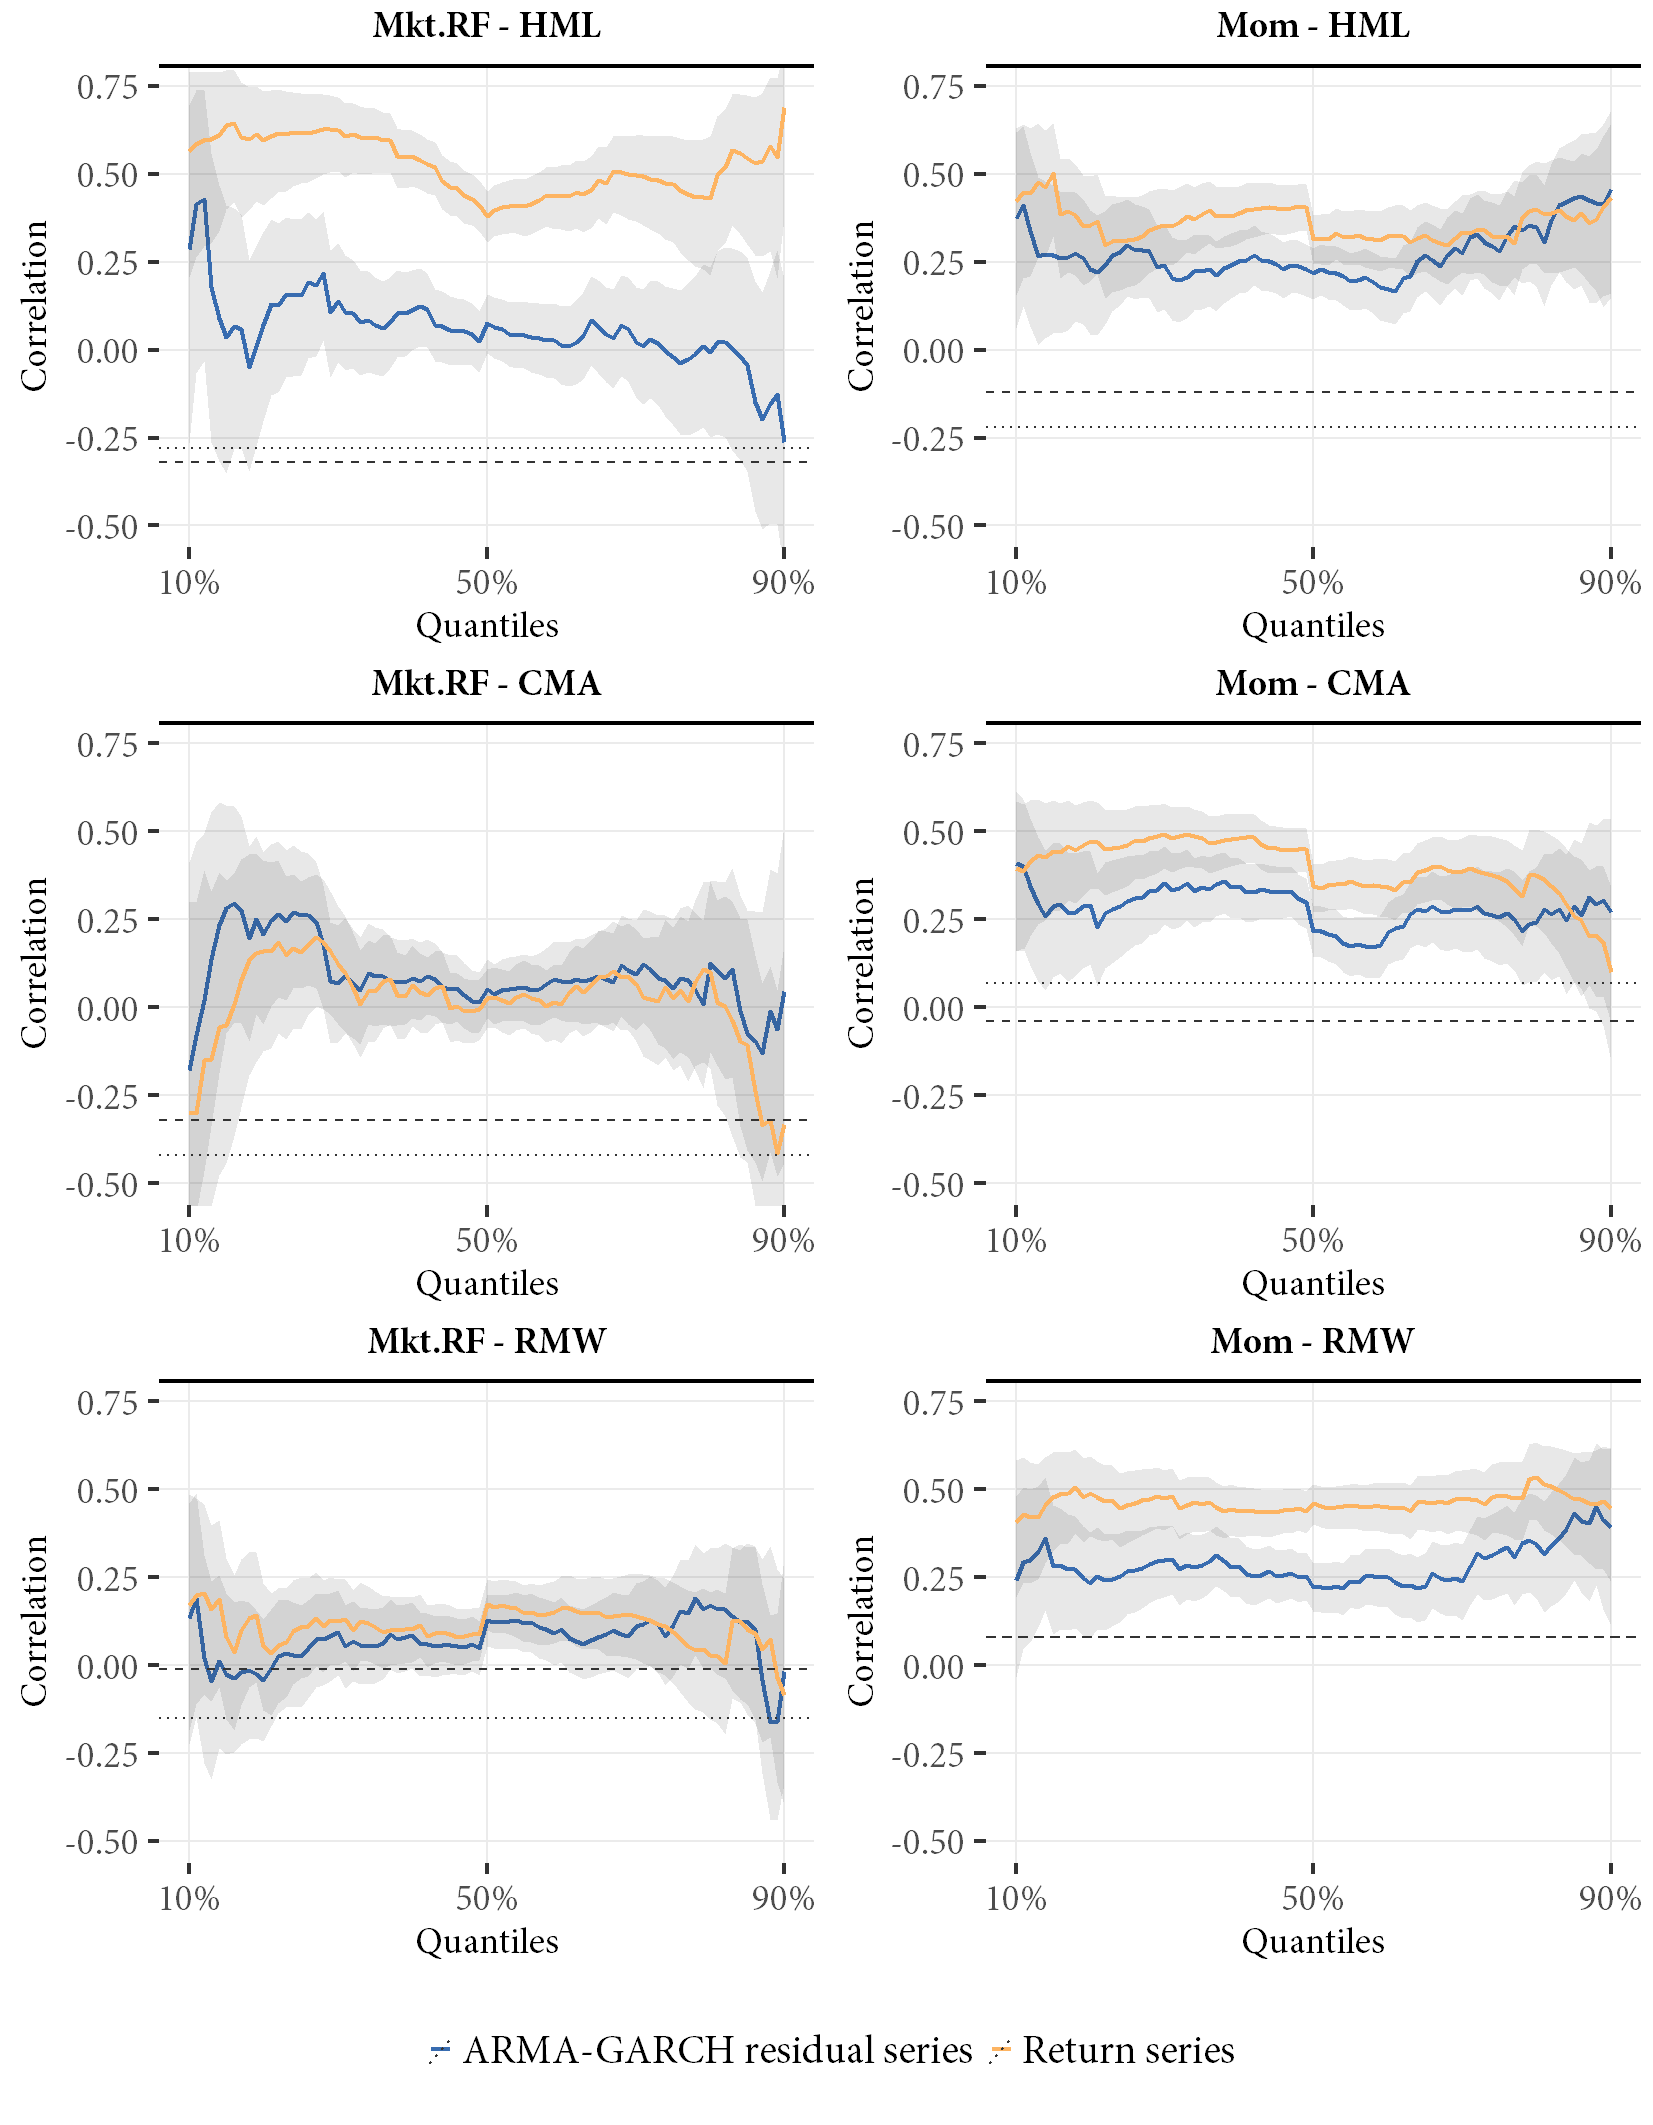
\includegraphics[scale=1]{graphics/appendix_threshold_1.png}  
\end{figure}
\begin{figure}[H]
  \centering
  \footnotesize
  \caption{Threshold correlations on returns as well as ARMA-GARCH residuals. Page 2/2 \\ \quad \\
  Threshold correlation plots with 95\% confidence bounds. Correlation pairs in graph titles. Unconditional correlations on returns and residuals given by the dashed lines. Weekly returns and ARMA-GARCH residuals from the chosen models, all data 1963--2016}
  \label{fig:appendix_threshold2}
  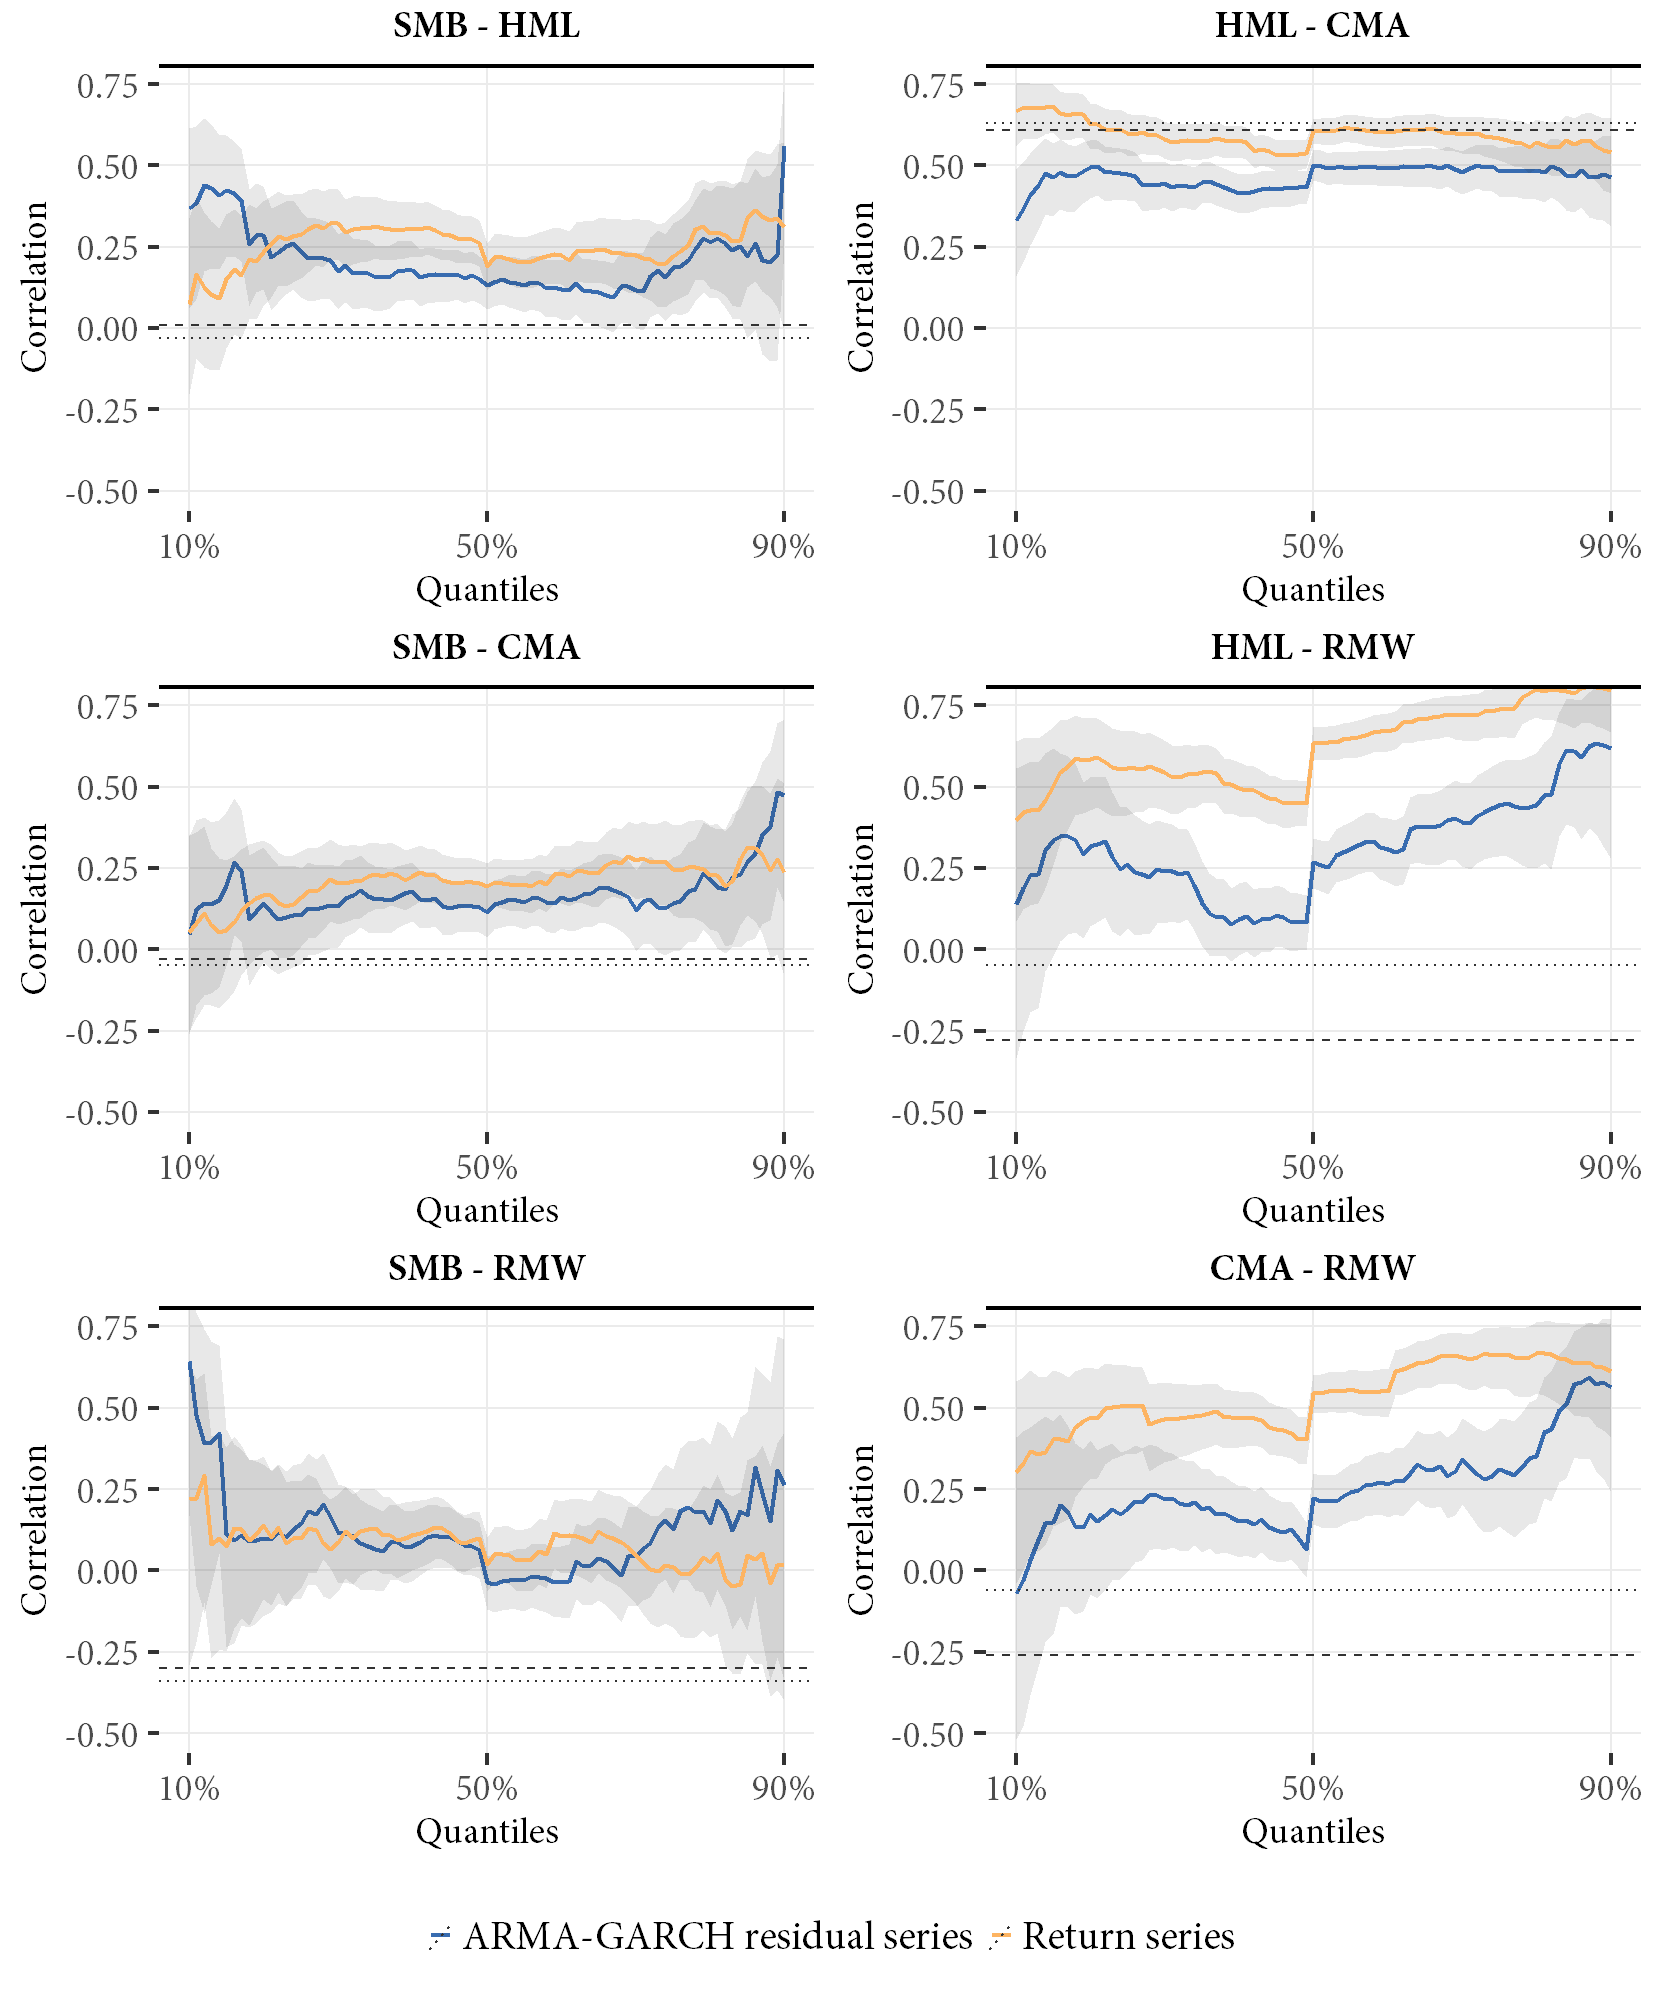
\includegraphics[scale=1]{graphics/appendix_threshold_2.png}  
\end{figure}

\newpage

\section{Rolling correlations on return series}
\label{app:rolling_return}
\begin{figure}[H]
  \centering
  \footnotesize
  \caption{Rolling correlations on returns as well as ARMA-GARCH residuals. Page 1/2  \\ \quad \\
  Rolling correlation plots with 95\% confidence bounds of both returns and ARMA-GARCH residuals. Correlation pairs in graph titles. Unconditional correlations on returns and residuals given by the dashed lines. Weekly returns and ARMA-GARCH residuals from the chosen models, all data 1963--2016}
  \label{fig:appendix_rolling1}
  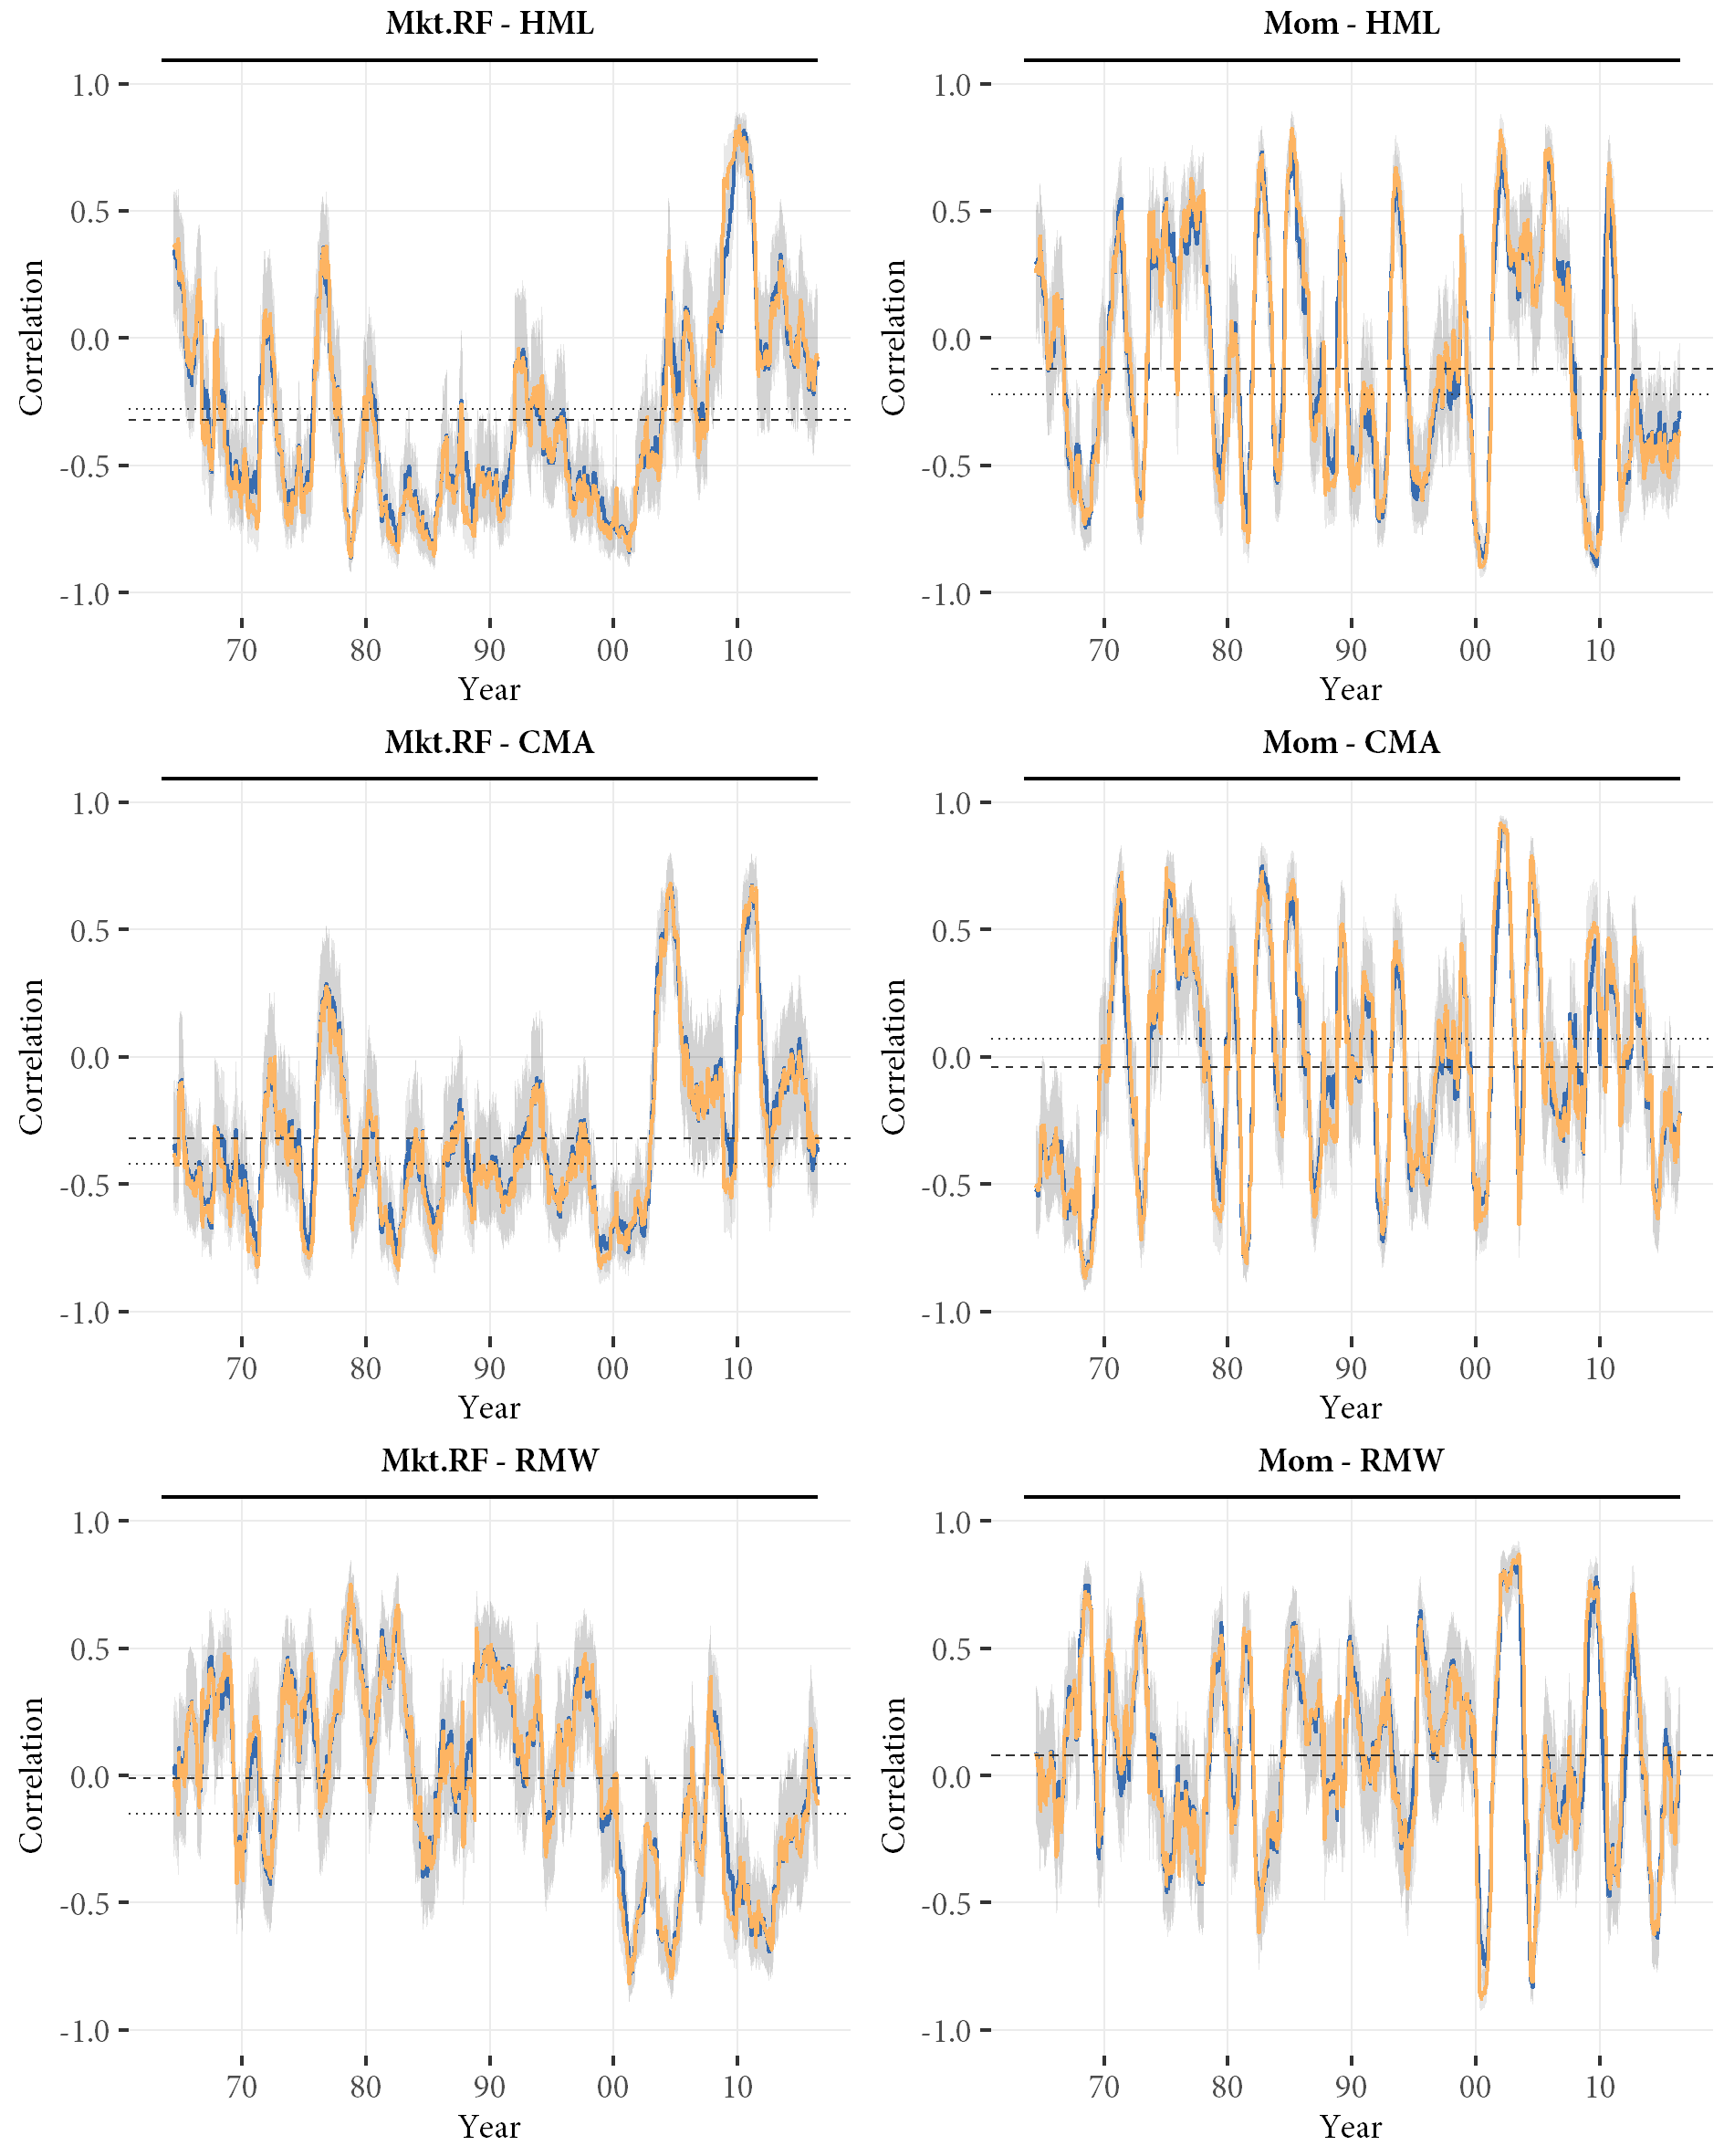
\includegraphics[scale=1]{graphics/appendix_rolling1.png}  
\end{figure}
\begin{figure}[H]
  \centering
  \footnotesize
  \caption{Rolling correlations on returns as well as ARMA-GARCH residuals. Page 2/2 \\ \quad \\
  Rolling correlation plots with 95\% confidence bounds of both returns and ARMA-GARCH residuals. Correlation pairs in graph titles. Unconditional correlations on returns and residuals given by the dashed lines. Weekly returns and ARMA-GARCH residuals from the chosen models, all data 1963--2016}
  \label{fig:appendix_rolling2}
  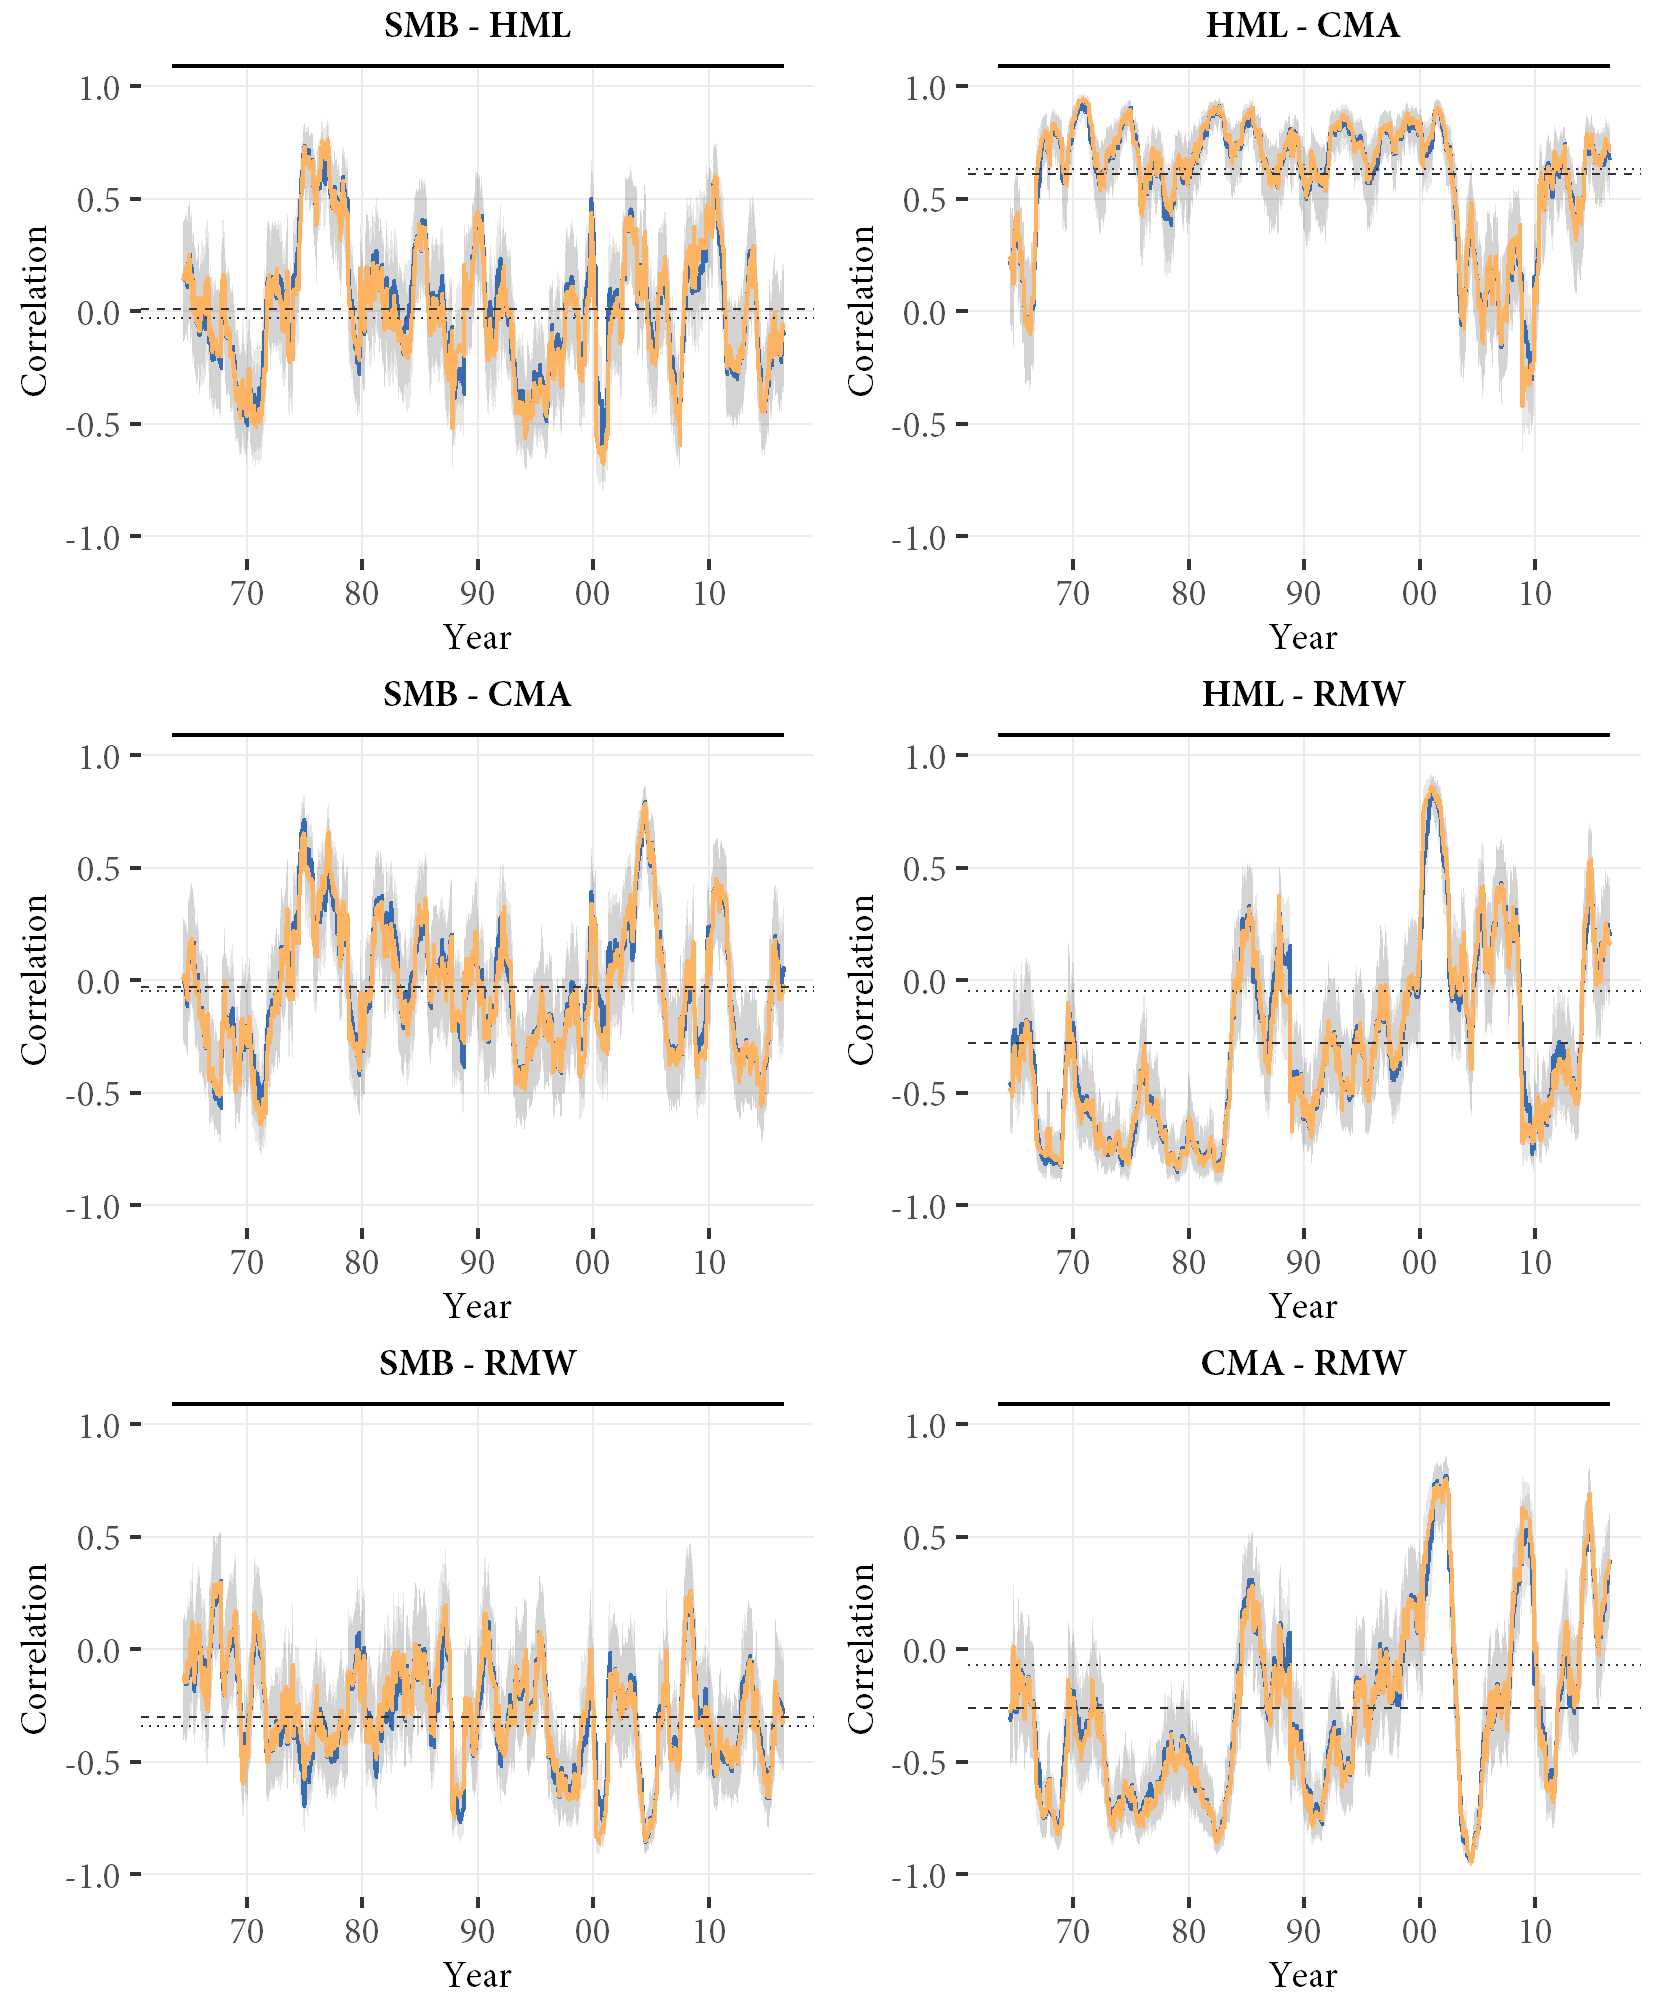
\includegraphics[scale=1]{graphics/appendix_rolling2.png}  
\end{figure}

\newpage

\section{Skewed Student's t distribution} 
\label{app:ghstmv}
We use the skewed Student's t distribution in modeling both univariate series as well as for the joint distribution under the copula. Both the normal and Student's t distributions can be considered special cases of this distribution. We use the definition of~\textcite{Hansen1994}.

Our description follows~\textcite{ChristoffersenLanglois2013}. A random vector $X$ that follows a multivariate skewed Student's distribution has the stochastic description
\begin{align}
  X = \sqrt{W}Z + \gamma W
\end{align}
where $\gamma$ is a vector of asymmetry parameters, $Z$ follows a standard multivariate normal distribution with correlation matrix $\Psi$, $W$ follows an inverse gamma distribution $\text{IG}(\dfrac{\nu}{2}, \dfrac{\nu}{2})$. Thus, the parameters of the multivariate distribution are degrees of freedom $\nu$, asymmetries $\gamma$ and an underlying correlation matrix $\Psi$.

The copula multivariate density function has the form:
\begin{align*}
  t_{\nu,\gamma,\Psi}(z_t^*) =
    & \frac{(\nu - 2)^\frac{\nu}{2} (\gamma^\top \Psi^{-1} \gamma)^{\frac{\nu+d}{2}}}{(2 \pi)^{\frac{d}{2}} |\Psi|^\frac{1}{2} \Gamma (\frac{\nu}{2}) 2^{\frac{\nu}{2} - 1}} \cdot \frac{K_{\frac{\nu + d}{2}} ( \sqrt{(\nu - 2 + Q(x)) \gamma^\top \Psi^{-1} \gamma}) e^{(x-\mu)^\top \Psi^{-1} \gamma} )}{( \sqrt{(\nu - 2 + Q(x)) \gamma^\top \Psi^{-1} \gamma})^{\frac{\nu + d}{2}}} 
\end{align*}

The random vector X is distributed multivariate generalized hyperbolic if
\begin{align}
    X \sim \mu + \sqrt{W} A Z + \gamma W
\end{align}
where $\mu$ is the location vector, $\gamma$ is the skewness vector, $R = A A^\top$ is the dispersion matrix, $W$ follows a generalized inverse-gamma distribution $W \sim GIG(\lambda, \chi, \psi)$ and Z is multivariate normal $Z \sim N(\mu^N, R)$, with $W, Z$ independent. The skewed Student-\textit{t} is nested with parameters
\begin{align}
    \lambda = \frac{\nu}{-2} && \chi = \nu - 2 && \psi = 0
\end{align}
where $\nu$ is the degree of freedom. Furthermore
\begin{align}
    \mathbb{E}[X] &= \mu + \mathbb{E}[W] \gamma \\
    Var[X] &= \mathbb{E}[Cov(X|W)] + Cov(\mathbb{E}[X|W]) \\
    &= Var(W) \gamma \gamma^\top + \mathbb{E}[W] R \nonumber
\end{align}
These moments describe the link between the copula correlation matrix $R$ and the skewed Student-\textit{t} distribution's dispersion matrix $R$. Covariances are finite when $\nu > 4$. The multivariate density function is given by
\begin{align} \label{eq:dskewt}
    f_X(x) &= \frac{(\nu - 2)^\frac{\nu}{2} (\gamma^\top R^{-1} \gamma)^{\frac{\nu+d}{2}}}{(2 \pi)^{\frac{d}{2}} |R|^\frac{1}{2} \Gamma (\frac{\nu}{2}) 2^{\frac{\nu}{2} - 1}} \cdot \frac{K_{\frac{\nu + d}{2}} ( \sqrt{(\nu - 2 + Q(x)) \gamma^\top R^{-1} \gamma}) e^{(x-\mu)^\top R^{-1} \gamma} )}{( \sqrt{(\nu - 2 + Q(x)) \gamma^\top R^{-1} \gamma})^{\frac{\nu + d}{2}}}
\end{align}
where $K(\cdot)$ is the modified Bessel function of the second kind, $Q(x) = (x-\mu)^\top R^{-1} (x-\mu)$, $d$ is the length of $x$, and $\Gamma$ is the gamma distribution density.

\newpage

\section{Copula Estimation Procedure} 
\label{app:copula_cdcc}

This is a step-by-step description of the procedure used to estimate the copula model, given the set of standardized residuals $\{z_{t}\}$ from each GARCH model. It is adapted from~\textcite{ChristoffersenErrunzaJacobLanglois2012} and uses the cDCC model of~\textcite{Aielli2013}.

For each week, compute uniform residuals by applying the probability integral transform to standardized residuals from each GARCH model:
\begin{align}
  u_{i, t+1} = \int_{-\infty}^{z_{i,t+1}} f_{i}(z_{i,t+1})
\end{align}
Note that while the distributions of returns is time-varying due to GARCH dynamics, the distribution of standardized returns is assumed constant, and in the case of skewed Student's t is parametrised by the shape $\nu_i$ and skewness parameter $\gamma_i$ (estimated as part of the GARCH models).

Transform the uniform residuals into copula residuals $z_{i,t+1}^*$ by applying the inverse cumulative distribution function of the copula to them:
\begin{align}
  z_{i,t+1}^* = F_{\nu_c,\gamma_i}^{-1}(u_{i,t+1})
\end{align}
Only under the normal copula will these residuals have expectation zero and unit variance -- hence, they are standardized by subtracting the expectation and dividing by the standard deviation of the distribution from~\autoref{app:ghstmv}.

These shocks are now used to fit the corrected DCC process of~\textcite{Aielli2013}. The correction involves the transformation $\bar{z}_{i,t+1}^* = z_{i,t+1}^* \sqrt{q_{ii,t}}$, where $q_{ii,t}$ are the diagonal elements of $Q_t$ and are found by a scalar version of~\autoref{eq:copula_cdcc}:
\begin{align}
  q_{ii,t} = (1 - \alpha - \beta)
    + \alpha (\bar{z}_{i,t-1}^*)^2
    + \beta q_{ii,t-1}
\end{align}
The corrected shocks are used to estimate the time-invariant component $Q$ using moment matching:
\begin{align}
  \hat{Q} = \frac{1}{T} \sum_{t=1}^T \bar{z}_{t}^* \bar{z}_t^{*\top}
\end{align}
Now, the full estimates of $\hat{Q}_t$ are computed using the sample estimate $\hat{Q}$ and the corrected shocks:
\begin{align}
  \hat{Q}_t = (1 - \alpha - \beta) \hat{Q}
    + \beta \hat{Q}_{t-1}
    + \alpha \bar{z}_{t-1}^* \bar{z}_{t-1}^{*\top}
\end{align}
The estimated $\hat{Q}_t$ matrices are standardized to estimates $\hat{\Psi}_t$ of the conditional correlation matrices of the copula using~\autoref{eq:copula_cdcc_psi}. When fitting the model, we thus choose parameters $\nu_c, \gamma_c, \alpha, \beta$ to generate $\hat{\Psi}_t$ which maximize the log-likelihood of observing copula shocks $z_t^*$ in each period.
% \subsection{Exogenous regressors in copula cDCC}
% It is relatively straightforward to make $S$ time-varying by adding a time-varying component $\Upsilon_t$ to it. Following the general case of~\autocite{ChristoffersenErrunzaJacobLanglois2012}, $\Upsilon_t$ is constructed from an $N\times(N + N_X)$ matrix $A$ where $N$ is the number of factors, and $N_X$ the number of explanatory variables. With the $N \times N_X$ matrix of coefficients $\theta$ and explanatory variables $X$, construct $A$ from an $NxN$ identity matrix and the element-wise multiplications of $\theta$ and $X$:
% \begin{align}
%   A &=
%     \begin{bmatrix}
%     1 & 0 & \cdots & 0            & \quad & \theta_{11} X_{11,t} & \cdots & \theta_{1N_X} X_{1N_X,t} \\
%     0 & 1 & \cdots & 0            & \quad & \theta_{21} X_{21,t} & \cdots & \theta_{2N_X} X_{2N_X,t} \\
%     \vdots & \vdots & \ddots & 0  & \quad & \vdots &               \vdots & \vdots \\
%     0 & 0 & \cdots & 1            & \quad & \theta_{N1} X_{N1,t} & \cdots & \theta_{NN_X} X_{NN_X,t}
%     \end{bmatrix}
% \end{align}
% Normalize $A$ by dividing each element with the root mean square of its row to ensure $\Upsilon_t$ is a correlation matrix:
% \begin{align}
%   \bar{A}_{ij} &= \frac{A_{ij}}{\sqrt{\sum_{k = 1}^{N + N_X} A_{ik}^2}}
% \end{align}
% Finally,
% \begin{align}
%   \Upsilon_t &= \bar{A} \bar{A}^\top
% \end{align}
% It is now straightforward to let e.g. $X_{ij} = t$ for a time-trend, or any other independent variable, common or asset specific. The new time-invariant component $\Omega$ should be estimated based on the sample averages of both the standardized shocks and $\Upsilon_t$. Replacing~\autoref{cdcc:momS} in the above list, we estimate $\hat{\Omega}$ as:
% \begin{align}
%   \hat{\Omega} &=
%     \frac{
%       \frac{1}{T} \sum^{T} z_t z_t^\top -
%       \phi
%       \frac{1}{T} \sum^{T} \Upsilon_t
%     }{1 - \phi}
% \end{align}

\newpage

\section{Stationary bootstrap of copula parameter standard errors} \label{App:Appendix_bootstrap}
We rely on the multi-step maximum likelihood estimation of the copula model, which takes the standardized residuals of marginal distributions as given in the second step. The first estimation step introduces parameter uncertainty that is not taken into account by the conventional standard errors of the second estimation.\footnote{Here, our model deviates from~\textcite{ChristoffersenLanglois2013}, who use a semi-parametric model that uses the empirical density function, and find standard errors using the analytical approach in~\textcite{ChenFan2006}. However, those errors are not valid in a time-varying copula context, as the estimation of means and variances impact the asymptotic distributions of copula parameters~\autocite{Remillard2010}.} We use the stationary block bootstrap method of \textcite{PolitisRomano1994} with a block length of 45 weeks (approx. 1 year of data) to find reliable standard errors for copula parameters. The procedure is theoretically supported by \textcite{GonclavesWhite2004} and implemented as follows:
\begin{enumerate}[(i)]
    \item Generate a block bootstrap version of the original weekly return data
    \item Estimate the ARMA-GJR-GARCH models and calculate standardized residuals
    \item Transform standardized residuals to uniform and estimate the copula model
    \item Collect the copula parameters $\Theta_i$
    \item Repeat (i)-(iv) N times to get $\{\Theta_i\}^{N}_{i=1}$
    \item Use the standard errors from the empirical distribution of $\{\Theta_i\}^{N}_{i=1}$
\end{enumerate}

\newpage

\section{Univariate diagnostic tests}
\label{app:univariate_diagnostics}

\textbf{Autocorrelation test}

The autocorrelation test is a weighted Ljung-Box test, following~\textcite{FisherGallagher2012} and~\textcite{LjungBox1978}. Under the null of a correctly specified model with no serial correlation, the weighted Ljung-Box test has been shown to generate results closer to its asymptotic distribution than the standard Ljung-Box test. The test statistic is given by
\begin{align}
  Q_W = T (T+2) \sum\limits^m_{k = 1} \frac{m-k+1}{m} \frac{\hat{r}_{k}^{2} (\hat{\epsilon}_{t} / \hat{\sigma}_{t})}{T-k}
\end{align}
where $T$ is the number of observations, $\hat{r}^{2}_{k} ( \hat{\epsilon}_{t} / \hat{\sigma}_{t} )$ is the squared sample autocorrelation of standardized residuals with lag order $k$ and max lag order $m$. Under the null, the test statistic is asymptotically distributed $\sum\limits^m_{k = 1} \chi^2_k \gamma_k$, where $\{\chi^2_k\}$ are independent chi-squared random variables with one degree of freedom and $\{\gamma_k\}$ are eigenvalues of a weighting matrix. We consider two maximum lag orders, 5 and 10 weeks. The maximum lag length was chosen by visual inspection of the autocorrelation functions for standardized residuals.

\textbf{Volatility clustering test}

For ARCH effects, we use the weighted LM test, following~\textcite{FisherGallagher2012} and~\textcite{LiMak1994}. The test has the null of no autocorrelation in standardized squared residuals from the model, and the test statistic is given by:
\begin{align}
  LM_W = T \sum\limits_{k = b + 1}^{m} \frac{m - k + (b+1)}{m} \hat{r}^{2}_{k} (\hat{\epsilon}^{2}_{t} / \hat{\sigma}_{t})
\end{align}
where $T$ is the number of observations, $b$ the number of autoregressive lags in the GARCH ($b=1$), $\hat{r}^2_k (\hat{\epsilon}^2_t / \hat{\sigma}_t)$ is the squared sample autocorrelation of standardized squared residuals with lag order $k$ and max lag order $m$. Under the null, the test statistic is asymptotically distributed $\sum\limits^m_{k = 1} \chi^2_k w_k$, where $\{\chi^2_k\}$ are independent chi-squared random variables with one degree of freedom and $\{w_k\}$ are the weighting parameters ($w = (m - k + (b+1))/m$). The maximum lag length was chosen by visual inspection of the autocorrelation functions for standardized squared residuals.

\textbf{Leverage effect test}

We use the sign bias test of~\textcite{EngleNg1993} to determine whether there are significant leverage effects in the factor returns. Run the regression
\begin{align}
  \hat{z}_t^2 = c_0 + c_1 I_{\hat{\epsilon}_{t-1} < 0} + c_2 I_{\hat{\epsilon}_{t-1} < 0} \cdot \hat{\epsilon}_{t-1} + c_3 I_{\hat{\epsilon}_{t-1} \geq 0} \cdot \hat{\epsilon}_{t-1} + u_t
\end{align}
where $\hat{z}_t^2$ are the standardized squared residuals of the ARMA-GARCH model, $I_\cdot$ are indicator functions that are equal to one when the subscript conditions are true, and $\hat{\epsilon}_{t-1}$ are the lagged ARMA-GARCH residuals. For the test of negative sign bias (i.e. leverage effect), the null hypothesis is $H_0: c_2 = 0$, and for the test of positive sign bias (i.e. reverse leverage effect), the null hypothesis is $H_0: c_3 = 3$. The Wald test statistics are asymptotically distributed $\chi^2$ with one degree of freedom.


